\documentclass[10pt,twocolumn,letterpaper]{article}

\usepackage{cvpr}
\usepackage{times}
\usepackage{epsfig}
\usepackage{graphicx}
\usepackage{amsmath}
\usepackage{amssymb}

\usepackage{url}
\usepackage{hyperref}

% Include other packages here, before hyperref.

% If you comment hyperref and then uncomment it, you should delete
% egpaper.aux before re-running latex.  (Or just hit 'q' on the first latex
% run, let it finish, and you should be clear).
%\usepackage[pagebackref=true,breaklinks=true,letterpaper=true,colorlinks,bookmarks=false]{hyperref}

\cvprfinalcopy % *** Uncomment this line for the final submission

\def\cvprPaperID{****} % *** Enter the CVPR Paper ID here
\def\httilde{\mbox{\tt\raisebox{-.5ex}{\symbol{126}}}}

% Pages are numbered in submission mode, and unnumbered in camera-ready
\ifcvprfinal\pagestyle{empty}\fi
\begin{document}

%%%%%%%%% TITLE
\title{PC-2020/21 Histogram Equalization}

\author{Lorenzo Arena\\
{\tt\small lorenzo.arena@stud.unifi.it}
}

\maketitle
\thispagestyle{empty}

%%%%%%%%% ABSTRACT
\begin{abstract}
    This project was made as the final work for the “Parallel Programming”
    exam at the University of Florence. The objective was to create three
    versions of a software to equalize the histogram of a given JPEG image.
    The first version had to be implemented as a sequential program, while
    the other two had to be parallel; for the parallel versions one has
    been implemented using OpenMP on top of the already implemented sequential
    code and the other is built using CUDA to take advantage of a GPU computing
    power. The projects has been developed in C on a Ubuntu machine; all
    tests were made on a Ryzen 7 1700 CPU and a NVIDIA Quadro P2000. The project
    is hosted on GitHub at \url{https://github.com/lorenzo-arena/histogram-equalizer}.
 \end{abstract}

 %%%%%%%%% BODY TEXT
\noindent\large\textbf{Future Distribution Permission}\\
\indent The author(s) of this report give permission for this document to be
        distributed to Unifi-affiliated students taking future courses.

\section{The algorithm}

%%%%%%%%%% TO WRITE
%% https://en.wikipedia.org/wiki/Histogram_equalization
Histogram equalization in image processing can be used to increase an image's
contrast. This is accomplished by spreading the most frequent intensities
values across the whole histogram. It works especially well on images which
presents foreground and background which are both dark or both bright.

\subsection{Implementation}

We can start by considering a grayscale image of \(n\) pixels, in which \(n_i\)
is the number of occurrences of gray level \(i\). The probability of an occurrance
of a pixel of level \(i\) (with \(0 < i < L\)) in the image is:

\[ p_x(i) = \frac{n_i}{n} \]

The histogram is the distribution of the pixel levels in the range \([0, L - 1]\).

We can define the \emph{cumulative distribution function} as the cumulative sum
of all the probabilities lying in its domain:

\[ cdf_x(i) = \sum_{j=0}^{i} p_x(x = j) \]

To get a linearized \(cdf\), which will produce a flatten histogram, we must
normalize the is to the \([0, L - 1]\) range by using the following formula:

\[ cdfn_x(i) = \frac{cdf(i) - cdf_{min}}{(M \cdot N) - cdf_{min}} \]

where \(M\) and \(N\) are the image's dimensions. The normalized \(cdf\) must
then be applied to the original histgram:

\[ h(v) = round(cdfn_x(i) \cdot (L - 1)) \]

While this can be applied to grayscale images by using the pixel value, for
color images applying the equalization process to the R, G and B channels would
break the image's color balance since the relative distribution of the color
channels would be changed. Thus, the pixels must be converted to another color
space (like HSL) where the algorithm can be applied to the \emph{luminance}
channel without creating changes in the \emph{hue} or \emph{saturation}
channels.

\subsection{On HSL color space}

HSL (\emph{hue}, \emph{saturation}, \emph{lightness}) is an alternative
representation of the RGB color space. Instead of describing colors by
using the red, green and blue components, it works by using a cylindrical
geometry where hue (the angular dimension) gives the description of the
perceived color (starting from red at 0°, green at 120° and blue at 240°).
Saturation describes the "colorfulness" of the color, giving the "pure color"
at value 1, at the edge of the cilinder, while turning to grayscale as the center
of the cilinder is approached. Lightness is used as the vertical axis dimension
and ranges from pure white (lightness 1) to pure black (lightness 0).

\begin{figure}[!ht]
    \centering 
    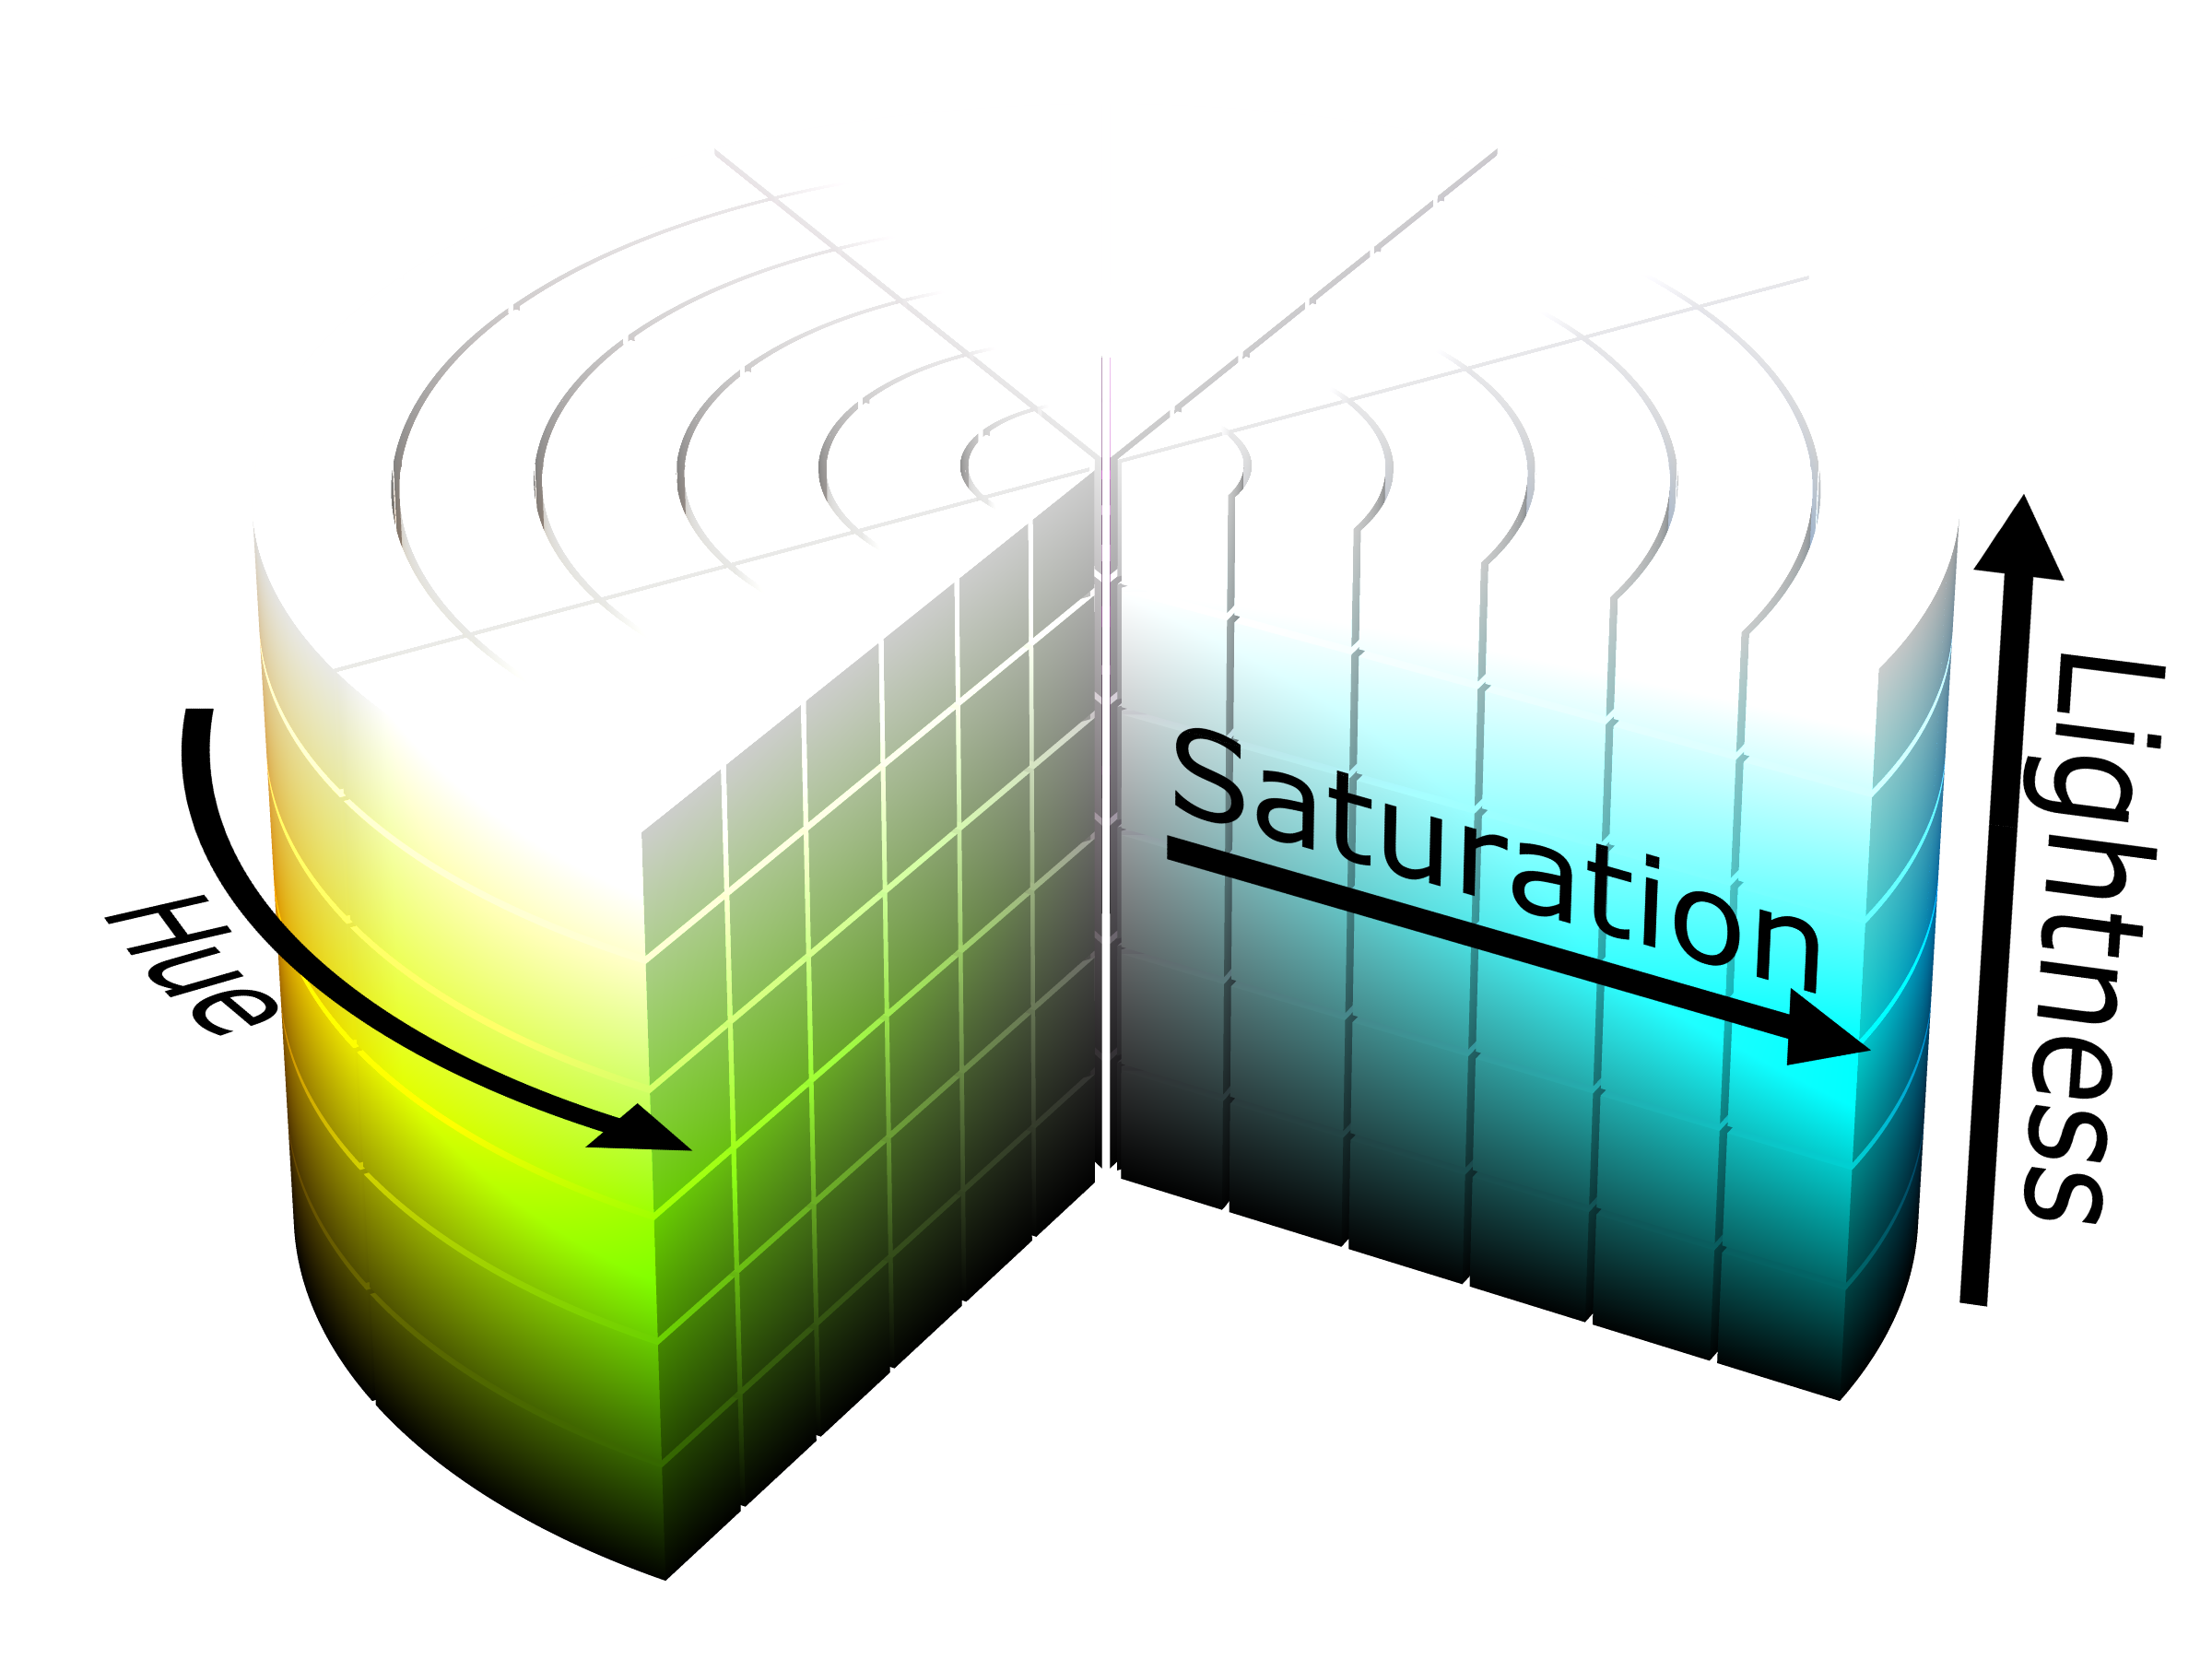
\includegraphics[width=0.8\linewidth]{./img/hsl.png}
    \caption{The HSL cilinder}
    \label{fig:hsl}
\end{figure}

\section{The sequential implementation}

The sequential solution was implemented by applying one by one all the algorithm
steps to an image which filename can be read from the command line when running
the program. The histogram is computed in 512 \emph{bins} for the luminance; by
using a special command line option it can also be printed out using \emph{gnuplot}.
The benchmarks have been made using \verb|clock_gettime| with \verb|CLOCK_MONOTONIC|,
both for getting a measure of the complete execution time (including image reading
from disk and output writing to disk) and for measuring the algorithm execution time.
The function to convert RGB pixels to HSL color space and viceversa has been
implemented following the process reported in \cite{wiki:HSL_and_HSV} under the
sections "\emph{From RGB}" and "\emph{To RGB}".

The tests were done on an image with low contrast, showed in Figure \ref{fig:input}.

\begin{figure}[!ht]
    \centering 
    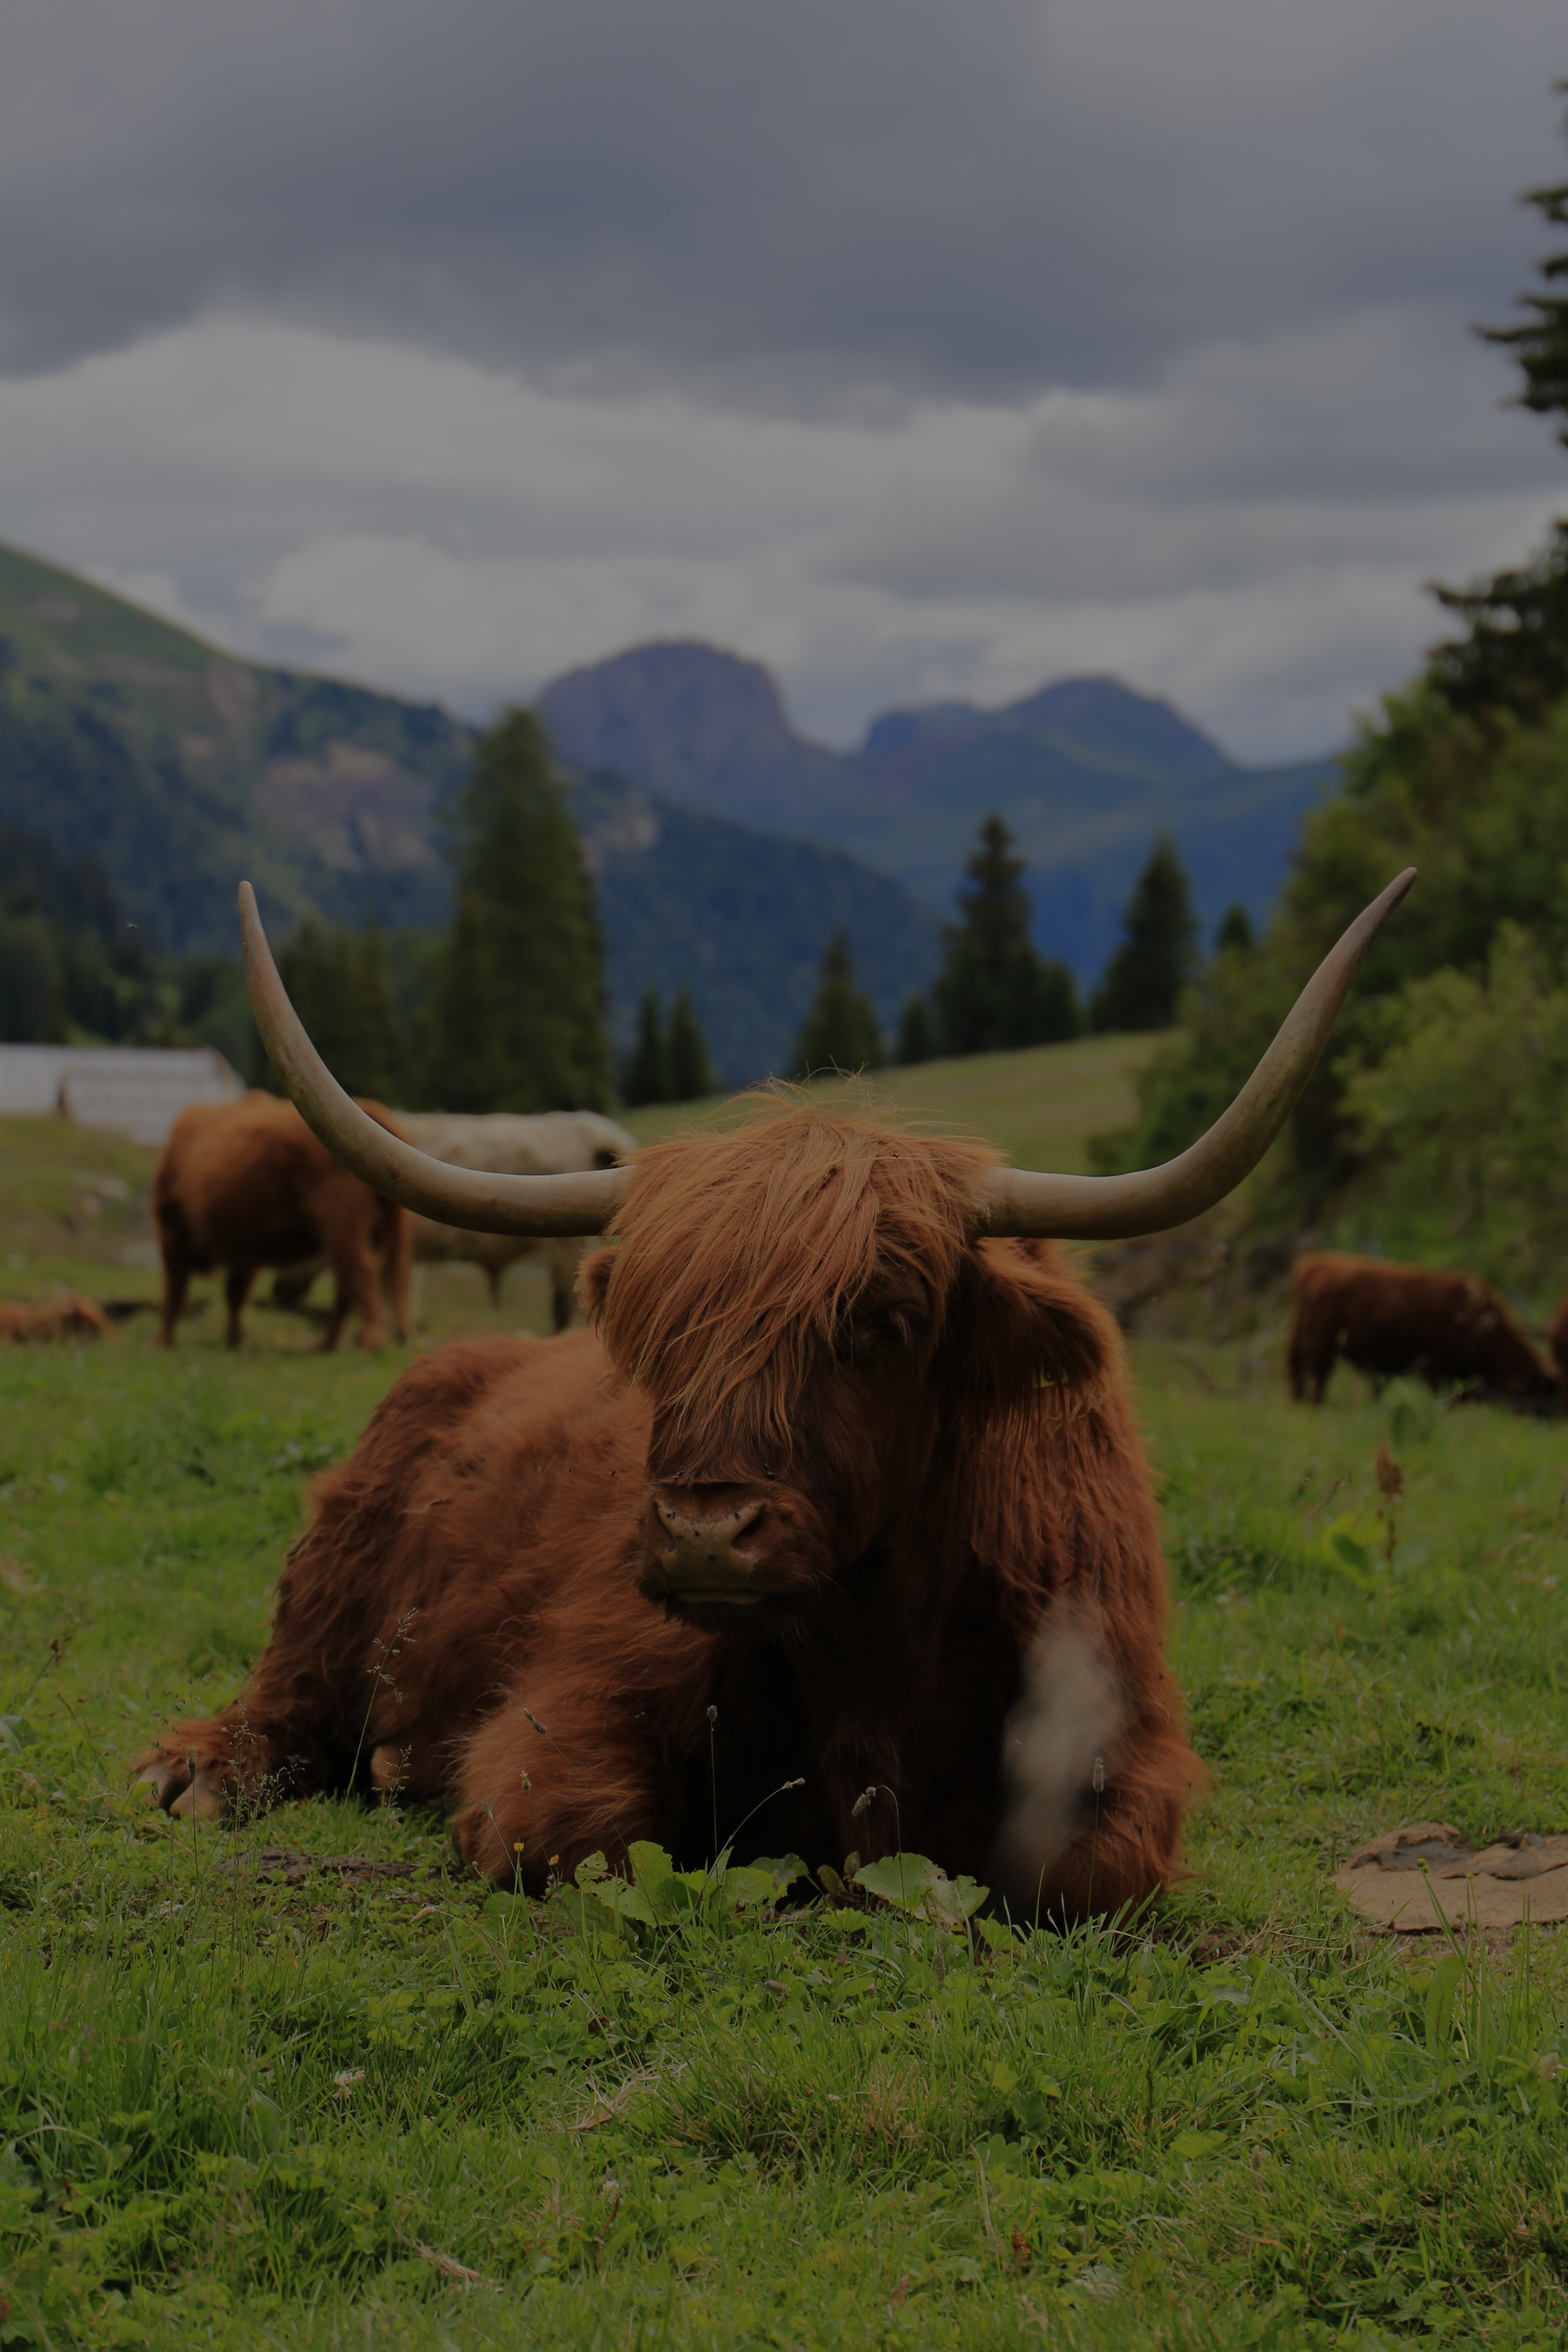
\includegraphics[width=0.8\linewidth]{../assets/pic_low_contrast.jpg}
    \caption{The test input image}
    \label{fig:input}
\end{figure}

The output after the equalization process is showed in Figure \ref{fig:output}.
The contrast has been increased, making the borders more clear while also darkening
the low lights on the animal body and lightening the high lights of the clouds.

\begin{figure}[!ht]
    \centering 
    \includegraphics[width=0.8\linewidth]{./img/output.jpg}
    \caption{The output image after the equalization process}
    \label{fig:output}
\end{figure}

\section{The OpenMP implementation}

\emph{OpenMP} is an API consisting of a set of compiler directives, libraries and
environment variables which can be used to develop parallel applications. It uses
a \emph{fork-join} model, where a primary thread forks a number of sub-threads and
divides a task between them. Each section of the code which is meant to be run in
a parallel fashion must be marked with a specific compiler directive; during the
execution each thread can get its \emph{id}, an integer which univocally identifies
it, with the function \verb|omp_get_thread_num|. Each thread executes the parallel
section independently, however there are a number of directives which allow
work sharing between threads, so that each one executes its allocated piece of work.
At the start of the program a thread pool is generated using the directive
\verb|#pragma omp parallel| (with a clause, or an option, to specify which variables
should be shared between the threads). Then, for each of the \verb|for| loops the
directive \verb|#pragma omp for| is used to split the work between the threads.
During the execution the directive \verb|#pragma omp single| is used to be sure that
only one thread executes memory allocations and other specific instructions.
Most of the equalization algorithm steps can be parallelized this way; the only exception
is the calculation of the cumulative distribution function, which is calculated from
a single thread.

The option \verb|-t| can be used when starting the OpenMP version of the program
to specify the number of threads which shall be used when performing the equalization.
By using that options some measures have been taken: the Figure \ref{fig:openmp-speedup}
shows the speedup of this implementation.

\begin{figure*}
\begin{center}
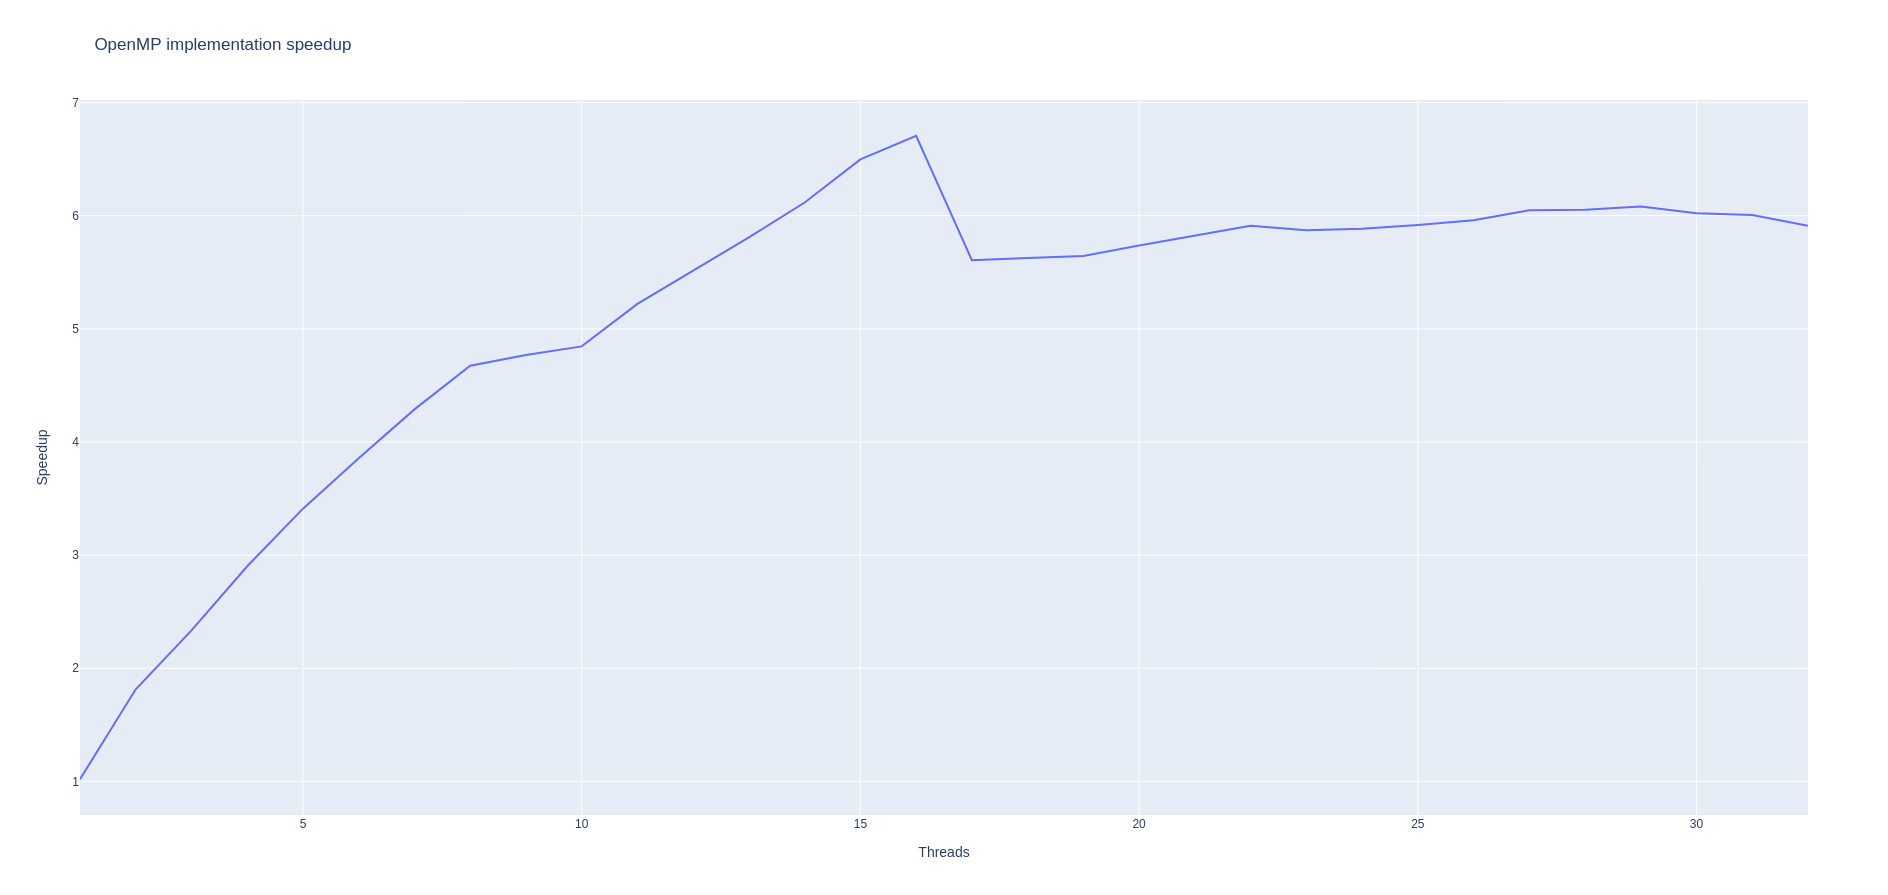
\includegraphics[width=1.0\linewidth]{./img/omp-speedup.png}
\end{center}
    \caption{The OpenMP implementation speedup}
\label{fig:openmp-speedup}
\end{figure*}

\section{The CUDA implementation}

The second parallel version of the software has been implemented using CUDA, thus being
able to take full advantage of a GPU computing power. The first approach was to transpose
each step of the algorithm to be run on the GPU; a \emph{kernel} (a routine compiled to be
executed on the GPU) has been implemented for each one of the equalization steps.
One of the first optimizations was related to the histogram computation: since there could
be potentially houndreds of threads writing to the same memory locations (that is, when
incrementing a "bin"), \emph{atomic} operations like \verb|atomicAdd| has been used; each
thread \emph{block} also works on a separate piece of memory, reducing the risk of collisions.
After some tests it has been chosen to use 30 \emph{blocks} of 512 threads each.
When the first implementation was completed it was noticed that one of the biggest bottlenecks
was the time necessary for the first \verb|cudaMalloc| call, which would take a lot of time
while the following CUDA function calls would take a lot less; it was probably relative to
the initialization of the runtime, and adding a simple \verb|cudaMalloc| and \verb|cudaFree|
for a 0 bytes array call at the start of the program contributed to trim that time.
Tables \ref{tbl:cuda-speedup-1} and \ref{tbl:cuda-speedup-2} reports the speedup of the
CUDA implementation for two images of different dimensions.

\begin{table}
    \begin{center}
    \begin{tabular}{|l|c|c|}
    \hline
    \multicolumn{3}{|c|}{Results for a 6MP image} \\
    \hline
    Implementation & Computation times & Speedup \\
    \hline
    Sequential: & 746ms & 1 \\
    OpenMP: & 114ms & 6.54 \\
    CUDA: & 25ms & 29.84 \\
    \hline
    \end{tabular}
    \end{center}
    \caption{CUDA results for 6MP image.}
    \label{tbl:cuda-speedup-1}
\end{table}

\begin{table}
    \begin{center}
    \begin{tabular}{|l|c|c|}
    \hline
    \multicolumn{3}{|c|}{Results for a 20MP image} \\
    \hline
    Implementation & Computation times & Speedup \\
    \hline
    Sequential: & 2386ms & 1 \\
    OpenMP: & 286ms & 8.34 \\
    CUDA: & 75ms & 31.81 \\
    \hline
    \end{tabular}
    \end{center}
    \caption{CUDA results for 20MP image.}
    \label{tbl:cuda-speedup-2}
\end{table}

\section{Results}

By using some utility scripts (which can be found in the repository) both for verifying
the correctness of the different solutions and to run them with different thread counts
(for the OpenMP implementation) or different input images, the following results are found:

\begin{itemize}
    \item the OpenMP implementation provides a good speedup over the sequential implementation;
          however, that stops getting better when the thread count is above the core count on
          which it is executed (or the virtual thread count in case of \emph{Simultaneous
          multithreading} enabled CPUs)
    \item for small images (under 6MP) both the OpenMP and the CUDA implementations provide a
          good speedup; however with bigger images the amount of parallelized computations grows
          while the not parallelized or not efficient (i.e. the scan computation) remains the same.
          This gets translated is an even higher speedup over the sequential implementation.
\end{itemize}

\newpage

\nocite{*}
\bibliography{project_report.bib} 
\bibliographystyle{ieee}

\end{document}